\section{Problem Overview}
The objective of this project is to develop a robust classification model capable of categorizing news articles into seven distinct classes: International News (0), Business (1), Technology (2), Entertainment (3), Sports (4), General News (5), and Health (6). The provided dataset consists of 79,997 labeled samples for training and development, and 20,000 additional samples for evaluation. Each entry includes metadata such as the source, title, timestamp, and PageRank score, along with the raw article content, which requires extensive preprocessing due to the presence of HTML tags.

\subsection{Data Distribution and Characteristics}
An exploratory data analysis (EDA) was conducted to understand the underlying structure of the dataset. As illustrated in Figure \ref{fig:label_distribution}, the class distribution is not perfectly uniform. While the dataset is relatively balanced, certain categories, such as Technology (Class 2), are overrepresented compared to others. This imbalance necessitates careful consideration during model training to prevent bias towards the majority classes.

\begin{figure}[h]
    \centering
    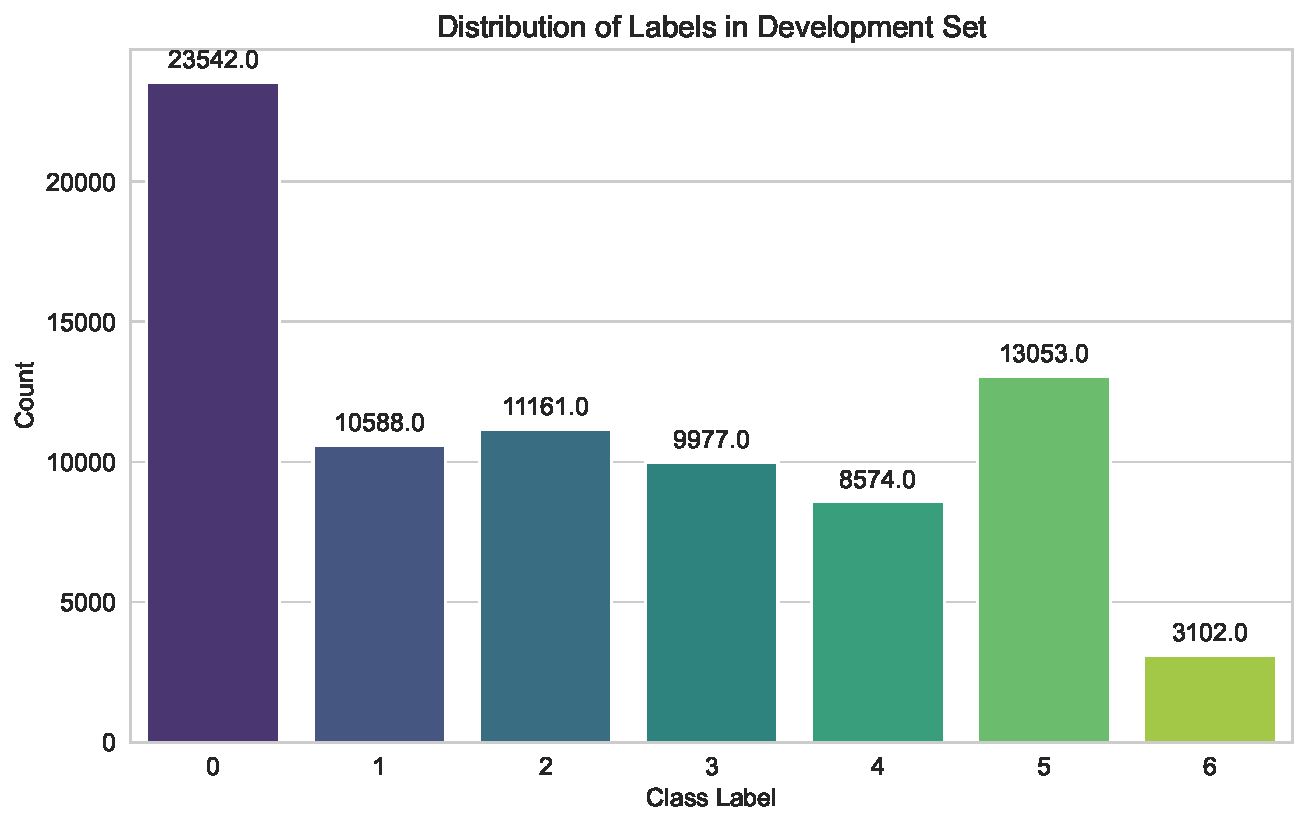
\includegraphics[width=0.8\textwidth]{final_img/plot_label_distribution.pdf}
    \caption{Distribution of class labels in the development set, highlighting the imbalance across categories.}
    \label{fig:label_distribution}
\end{figure}

Another critical observation concerns the lexical similarity between categories. We analyzed the number of shared terms among the top 100 most frequent words for each class. As depicted in the heatmap in Figure \ref{fig:common_words}, International News (Class 0) and General News (Class 5) exhibit a notable overlap in their vocabulary. This substantial intersection suggests a semantic proximity that may introduce ambiguity, complicating the classification task for models relying solely on simple bag-of-words representations.

\begin{figure}[h]
    \centering
    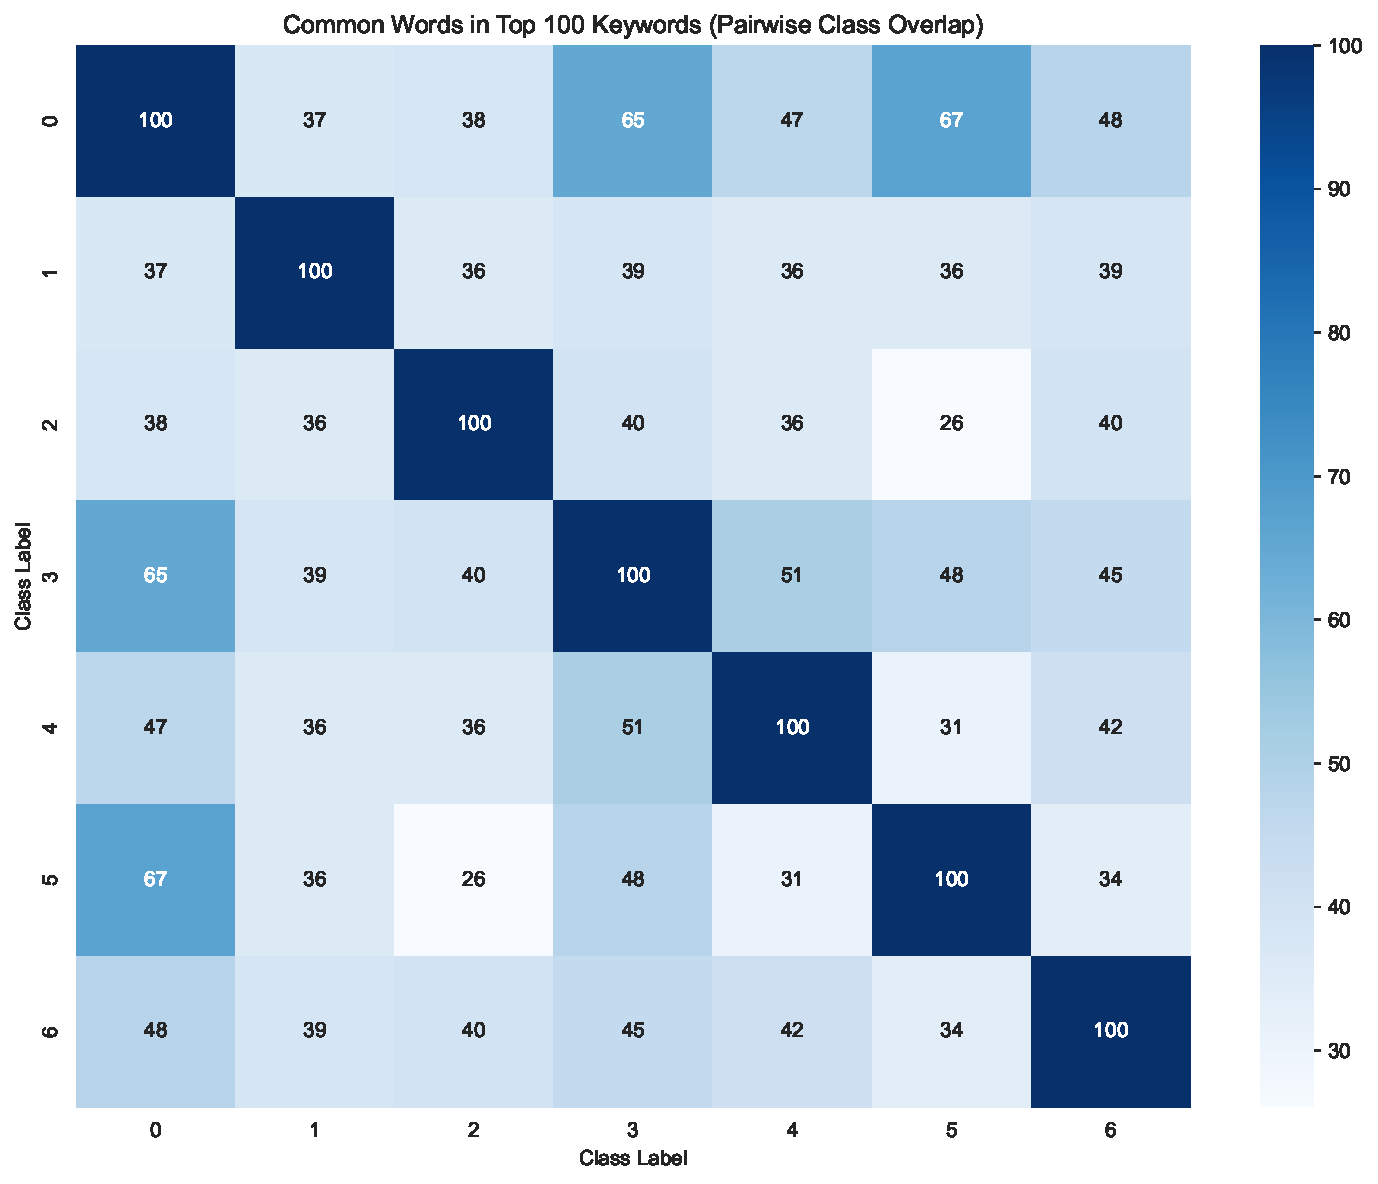
\includegraphics[width=0.8\textwidth]{final_img/common_words_matrix.pdf}
    \caption{Pairwise intersection of the top 100 most frequent words across classes. The heatmap highlights significant lexical overlap between specific category pairs, particularly Class 0 and Class 5.}
    \label{fig:common_words}
\end{figure}

Additionally, we analyzed the distribution of article lengths (word count) across different categories to identify potential discriminative features. The length of the articles varies significantly by topic, as detailed in Table \ref{tab:word_counts}. For instance, Technology articles (Class 2) are generally the longest, with a mean length of approximately 44.8 words and a high standard deviation (88.6), indicating significant variability and the presence of outliers (max 1905 words). Conversely, General News articles (Class 5) are the shortest on average (24.9 words) with the lowest maximum length (77 words). This distinct variation suggests that article length is a valuable feature for differentiating between certain classes.

\begin{table}[h]
\centering
\begin{tabular}{lrrr}
\hline
\textbf{Label} & \textbf{Mean Length} & \textbf{Std Dev} & \textbf{Max Length} \\ \hline
0 (International News) & 37.27 & 23.46 & 403 \\
1 (Business) & 27.75 & 16.67 & 184 \\
2 (Technology) & 44.76 & 88.63 & 1905 \\
3 (Entertainment) & 34.74 & 21.10 & 290 \\
4 (Sports) & 35.72 & 18.15 & 243 \\
5 (General News) & 24.91 & 12.00 & 77 \\
6 (Health) & 32.46 & 16.28 & 190 \\ \hline
\end{tabular}
\caption{Statistics of article word counts across different categories.}
\label{tab:word_counts}
\end{table}
Finally, we investigated the relationship between news sources and article categories. Our analysis revealed that certain publishers demonstrate a high degree of topic specificity. As illustrated in Figure \ref{fig:pure_sources}, specific sources are almost exclusively associated with a single category (e.g., 'ESPN' with Sports, 'PCWorld' with Technology). This high "purity" implies that the 'source' attribute contains significant predictive signal. Consequently, incorporating source information—potentially with increased weight or through specific feature engineering—is likely to substantially enhance the classifier's performance for these subsets of data.

\begin{figure}[h]
    \centering
    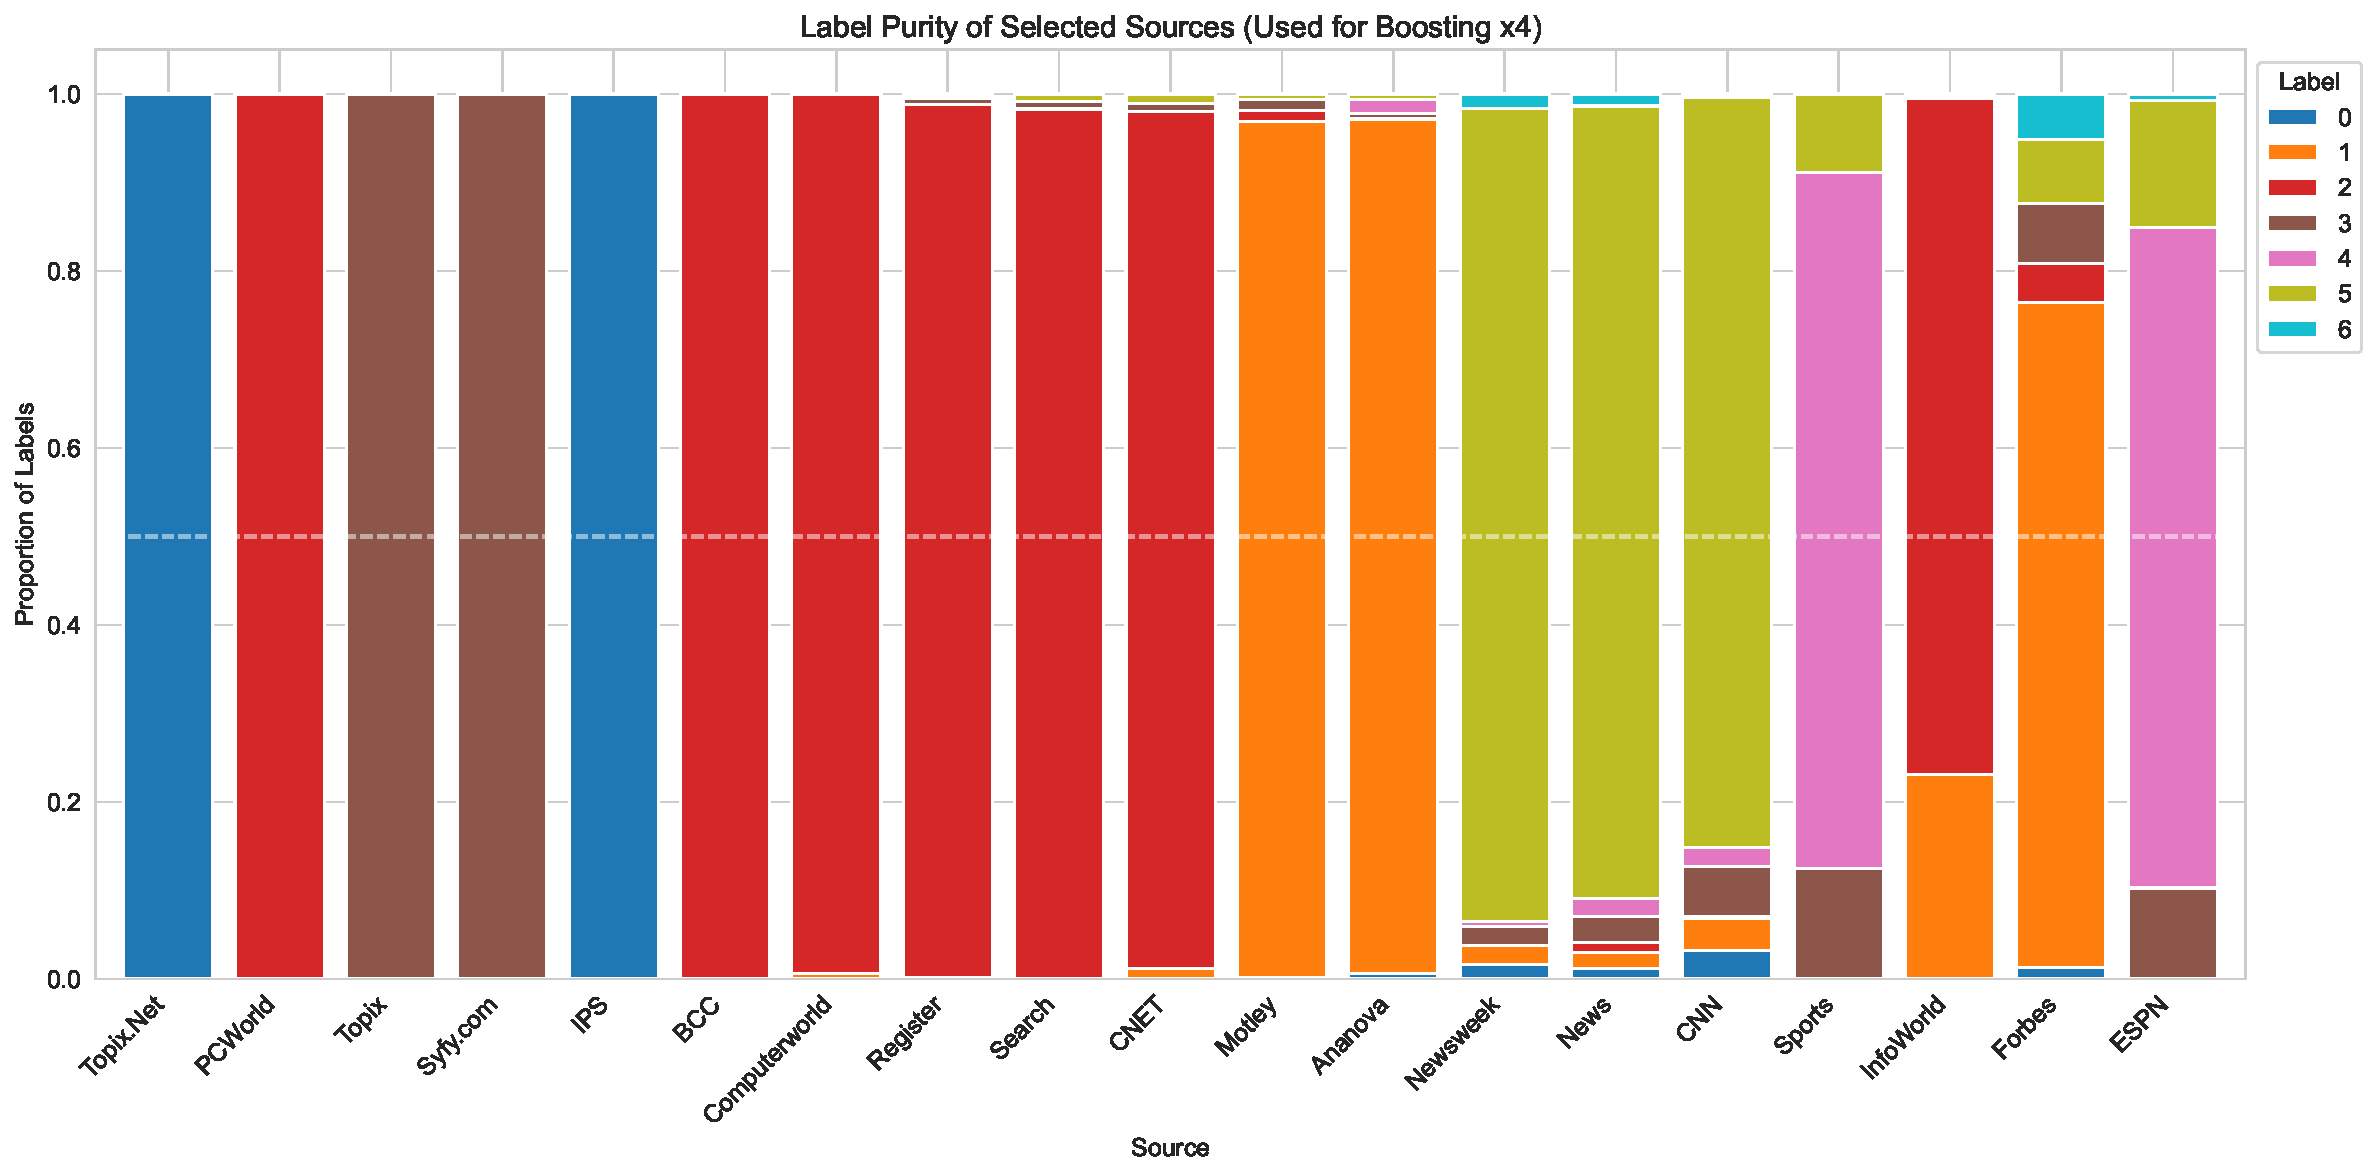
\includegraphics[width=0.8\textwidth]{final_img/plot_pure_sources.pdf}
    \caption{Label purity of selected news sources. High purity indicates that a source predominantly publishes articles of a single category, making it a strong predictive feature.}
    \label{fig:pure_sources}
\end{figure}
